\documentclass{article}

% Official NeurIPS 2026 style (dblblindworkshop track).
% Source: https://media.neurips.cc/Conferences/NeurIPS2026/Formatting_Instructions_For_NeurIPS_2026.zip
% linked from https://neurips.cc/Conferences/2026/CallForPapers ("Paper template").
% neurips_2026.sty SHA-256:
% c3fc2894e83d2517ca18b66741d6c595986d97957dc08ec08bb2125a7ec4555a
% Retrieved 2026-07-24T18:17:44Z. Main-track checklist.tex is intentionally
% not loaded (GDDL CFP does not require it).
\usepackage[dblblindworkshop]{neurips_2026}
\workshoptitle{Geometric Distributional Deep Learning: Bridging Optimal Transport, Learning and Structured Data}

\usepackage[utf8]{inputenc}
\usepackage[T1]{fontenc}
\usepackage{hyperref}
\hypersetup{
  hidelinks,
  pdftitle={},
  pdfauthor={},
  pdfsubject={},
  pdfkeywords={},
}
\usepackage{url}
\usepackage{booktabs}
\usepackage{amsmath,amssymb,amsthm}
\usepackage{graphicx}
\usepackage{microtype}
\usepackage{enumitem}
\AtBeginDocument{%
  \setlength{\abovedisplayskip}{5pt plus 1pt minus 2pt}%
  \setlength{\belowdisplayskip}{5pt plus 1pt minus 2pt}%
  \setlength{\abovedisplayshortskip}{3pt plus 1pt}%
  \setlength{\belowdisplayshortskip}{3pt plus 1pt}%
}

\newtheorem{proposition}{Proposition}

\newcommand{\wtwo}{W_2}
% Anonymized audit-artifact aliases; the mapping to full artifact IDs,
% checksums, and config hashes ships in the supplementary alias manifest.
\newcommand{\artifact}[1]{\textsf{\small #1}}

\title{When Averaged Field Regularity Fails to Rank\\ Few-Step Generative Paths}

\author{%
  Anonymous Author(s)\\
}

\begin{document}

\maketitle

\begin{abstract}
Choosing a probability path for few-step generative sampling is often
guided by averaged regularity of the velocity field: a path with smaller
averaged squared Jacobian norm is expected to discretize better at a
fixed budget of function evaluations (NFE). We study this question in
commuting Gaussian
flows, where endpoint laws and Gaussian 2-Wasserstein ($\wtwo$) errors
are available in closed form and the regularity integrand is analytically
known; sampling, training, and estimation noise are absent. The
averaged-regularity ordering of linear versus variance-preserving paths
fails to determine the fixed-NFE $\wtwo$ ordering: fourteen inversions
identified in a registered benchmark reproduce in a frozen clean-code
grid across Euler, Heun, and RK4, survive an 80-digit precision audit,
and recur in a separately pre-registered non-centered replication
family. An exact modal decomposition expresses the mismatch through solver-stage
sampling and signed one-step defects transported to the endpoint; an
explicit scalar construction proves the non-implication for fixed-grid
Euler. Pairwise linear-versus-VP ranking is not a substitute for an
in-family objective: even among shared $(\alpha,\sigma)$ interpolants the
unsigned average need not order equal-NFE $\wtwo$, and the unconstrained
per-mode minimizer is not a shared interpolant for $d\geq 2$. No learned
model is evaluated.
\end{abstract}

\section{Introduction}

Few-step sampling of continuous-time generative models commits to a
probability path, a solver, and a small NFE budget before any error is
observed. Lipschitz and stability constants enter classical
numerical-error bounds~\citep{hairer1993solving}, and
\citet{lipschitzguided2025} propose averaged squared drift Lipschitzness
as a schedule criterion; bounding an error, however, is weaker than
determining which of two paths errs less at an equal small budget. We
isolate that question where the marginal flow is affine, the fixed-step
endpoint law follows in closed form, and the error is the closed-form
Gaussian $\wtwo$~\citep{gelbrich1990formula}; reported values are
checked against an 80-digit reference.

\textbf{Contributions.}
\begin{itemize}[leftmargin=1.4em,itemsep=1pt,topsep=2pt]
  \item A controlled closed-form $\wtwo$ benchmark on commuting
  Gaussian flows: fourteen inversions identified in a registered
  benchmark reproduce in a frozen clean-code grid (14 of 36 comparisons,
  80-digit-verified), and a separately pre-registered non-centered
  replication family shows the same phenomenon (11 of 18).
  \item An exact eigenmode analysis: the endpoint factor error is a
  transported sum of signed, solver-stage-dependent local defects, which
  an unsigned time average of Jacobian norms cannot retain.
  \item An explicit grid-aware smooth scalar construction proving that, for every
  $L>0$ and grid size $N$, strictly larger averaged squared Jacobian is
  compatible with zero fixed-grid Euler endpoint error.
\end{itemize}

Solver dependence of good schedules is not itself
novel~\citep{sabour2024align,karras2022edm}; the contribution is the
exact, controlled non-implication and its modal explanation, bounding
what averaged regularity certifies about fixed-budget \emph{rankings}
in the tested systems.

\begin{figure}[t]
  \centering
  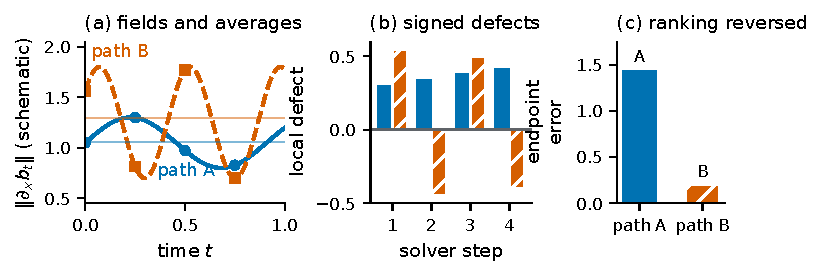
\includegraphics[width=\linewidth]{figures/fig1_conceptual.pdf}
  \caption{\textbf{Conceptual schematic, not experimental data.}
  (a)~Averaging collapses two time-dependent fields to two scalars, while
  a solver samples only stage locations (dots and squares). (b)~Local
  defects are signed: same-sign defects accumulate, alternating defects
  cancel. (c)~Transported to the endpoint, the error ranking can oppose
  the averaged ranking. This illustrates the accounting of
  Section~\ref{sec:mechanism}, not the measured mechanism of any
  specific Gaussian inversion.}
  \label{fig:concept}
  \vspace{-6pt}
\end{figure}

\section{Gaussian probability flows and averaged regularity}
\label{sec:setup}

Let $X_0\sim N(\mu_0,\Sigma_0)$ and $X_1\sim N(\mu_1,\Sigma_1)$ be
independent and let a scalar schedule $(\alpha(t),\sigma(t))$, with
$\alpha(0)=\sigma(1)=1$ and $\alpha(1)=\sigma(0)=0$, define the interpolant
$X_t=\alpha X_0+\sigma X_1$~\citep{albergo2025stochastic,lipman2023flow}.
The marginal law is Gaussian with mean $m_t=\alpha\mu_0+\sigma\mu_1$ and
covariance $Q(t)=\alpha^2\Sigma_0+\sigma^2\Sigma_1$, and the marginal
velocity field is affine,
\begin{equation}
  b(t,x)=A(t)\,x+c(t),\qquad
  A(t)=C_t\,Q(t)^{-1},\qquad
  c(t)=\dot m_t-A(t)\,m_t,
  \label{eq:affine}
\end{equation}
with $C_t=\dot\alpha\alpha\,\Sigma_0+\dot\sigma\sigma\,\Sigma_1$; centered
with $\Sigma_0=I$ this is $A(t)=\tfrac12 Q'Q^{-1}$, $c\equiv0$. We
compare the \emph{linear} path $(1-t,\,t)$ and the trigonometric
\emph{variance-preserving} (VP) path
$(\cos\tfrac{\pi t}{2},\,\sin\tfrac{\pi t}{2})$, the interpolant
analogue of VP diffusion schedules (background:
\citealp{song2021score}). Following \citet{lipschitzguided2025}, the
baseline is $\mathcal{R}[b]=\int_0^1\|A(t)\|_2^2\,dt$, evaluated by
trapezoidal quadrature of the analytically known spectral-norm
integrand; by its own definition $\mathcal{R}$ ignores $c(t)$. Error is
Gaussian $\wtwo$, the closed-form distribution-level metric of this
schedule-design literature.

A fixed-step solver applied to \eqref{eq:affine} induces an affine
endpoint map, reconstructed from $d{+}1$ deterministic probes; pushing
the source moments through it and applying the closed-form Gaussian
$\wtwo$~\citep{gelbrich1990formula} gives the endpoint error (float64,
verified against an 80-digit reference below). With
$\Sigma_0=I$ and $\Sigma_1=U\mathrm{diag}(\lambda_i)U^{\top}$ all matrices
commute: each mode obeys $x_i'=a_i(t)x_i+c_i(t)$ with $a_i=q_i'/(2q_i)$,
$q_i=\alpha^2+\sigma^2\lambda_i$, and centered,
$\wtwo^2=\sum_i(|r_i|-\sqrt{\lambda_i})^2$ with $r_i$ the product of the
numerical one-step factors of mode $i$.

\section{Why the ranking need not agree: transported signed defects}
\label{sec:mechanism}

The exact one-step transition of mode $i$ over $[t_n,t_{n+1}]$ is
$e_{i,n}=\sqrt{q_i(t_{n+1})/q_i(t_n)}$, while a Runge--Kutta step
multiplies by a factor $r_{i,n}$ built from stage samples of $a_i$ (one for
Euler, two for Heun, four for RK4). For smooth $a$, the leading coefficients
of the local defect (exact minus method) are $\tfrac12(a'+a^2)h^2$ for Euler
and $(-\tfrac1{12}a''+\tfrac16a^3)h^3$ for Heun---different derivatives, signs,
and stage locations. With $S$ the number of steps, the endpoint factor error
obeys the exact telescoping identity
\begin{equation}
  \prod_{n<S}r_{i,n}-\prod_{n<S}e_{i,n}
  =\sum_{n<S}(r_{i,n}-e_{i,n})
  \Bigl(\prod_{j<n}r_{i,j}\Bigr)\Bigl(\prod_{j>n}e_{i,j}\Bigr),
  \label{eq:telescope}
\end{equation}
with no smallness or positivity assumption. This identifies what
$\mathcal{R}$ discards: which times the stages sample, the derivatives
of $A$, the \emph{signs} of local defects, their cancellation, and their
transport to the endpoint---so an unsigned average of $\|A\|^2$ need not
determine the fixed-NFE ordering.

\section{Controlled benchmark and results}
\label{sec:results}

\textbf{Design and chronology.} Source $N(0,I)$; anisotropic (condition
number 4) and seeded low-rank ($FF^{\top}{+}0.05I$, rank 2) targets;
$d\in\{2,8\}$; linear and VP paths; Euler, Heun, RK4; NFE
$\in\{8,16,32\}$ with equal-NFE accounting (steps $=$ NFE$/$stages): 72
float64 CPU configurations in 36 two-path blocks. A \emph{ranking
inversion} is a block where the $\mathcal{R}$ and $\wtwo$ orderings
strictly disagree. The inversions were first identified in a registered
benchmark, then the grid above was frozen and rerun from clean code;
post-hoc diagnostics are labeled as such.

\textbf{Fourteen audited inversions.} All 72 configurations reproduce
the registered run within $10^{-12}$; 14 of 36 blocks are inversions
(Figure~\ref{fig:inversions}; audit artifact \artifact{A1}). In the
strongest, low-rank at $d=8$ with Euler at NFE 8
(Table~\ref{tab:strongest}), the baseline prefers linear whose $\wtwo$
is $78\%$ larger (margin $0.3543761036$). All 72 float64 $\wtwo$ values
agree with an 80-digit \texttt{mpmath} reference to at most
$9.71\times10^{-10}$; the smallest inversion margin,
$1.1189\times10^{-5}$, exceeds this 11{,}500-fold (artifacts
\artifact{A1}--\artifact{A2}).

\begin{table}[t]
  \centering
  \caption{Strongest inversion: low-rank Gaussian, $d=8$, Euler, NFE 8
  (artifact \artifact{A1}).}
  \label{tab:strongest}
  \begin{tabular}{lcc}
    \toprule
    path & $\mathcal{R}[b]$ (lower = preferred) & Gaussian $\wtwo$\\
    \midrule
    linear & $\mathbf{2.9476523251}$ & $0.8108540111$\\
    variance-preserving & $4.7295206355$ & $\mathbf{0.4564779075}$\\
    \bottomrule
  \end{tabular}
\end{table}

\begin{figure}[t]
  \centering
  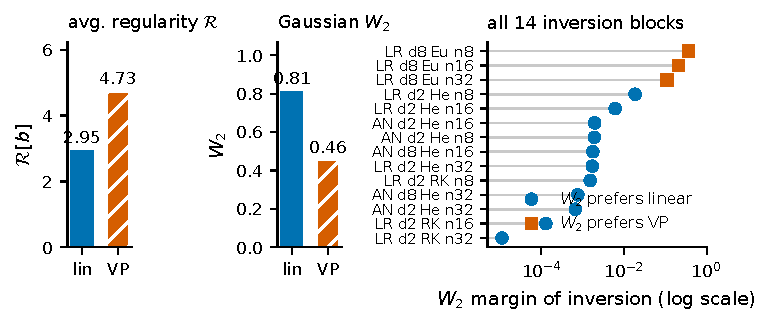
\includegraphics[width=\linewidth]{figures/fig2_inversions.pdf}
  \caption{\textbf{Left:} the strongest inversion in both quantities;
  hatching marks VP. \textbf{Right:} $\wtwo$ margins of all fourteen
  inversion blocks on a logarithmic axis (which compresses, never
  exaggerates, magnitudes); marker shape and color give the
  $\wtwo$-preferred path (artifact
  \artifact{A1}).}
  \label{fig:inversions}
  \vspace{-6pt}
\end{figure}

\textbf{Solver--path interaction.} In the low-rank grid, VP is preferred
under Euler and linear under Heun and RK4, at both dimensions and every
primary budget (Figure~\ref{fig:interaction}); the pattern persists at
NFE 64 and 128 and under $\pm10\%$ target perturbations (artifact
\artifact{A4}). Solver-dependent schedule preference is
established~\citep{sabour2024align}; here, the tested
averaged-regularity scalar does not capture this interaction.

\textbf{Pre-registered non-centered replication.} Before execution we
froze one supporting family: source $N(\mu_0,I)$,
$\mu_{0,i}=0.75(-1)^i$; target $N(\mu_1,D)$, $\mu_{1,i}=1+0.25i$, $D$
geometric with condition number 6---so $c(t)\neq0$ in
\eqref{eq:affine}---with the same paths, solvers, and budgets. Eleven of
eighteen blocks are inversions ($\mathcal{R}$, which ignores $c(t)$ by
definition, prefers VP with margin $0.7513$; $\wtwo$ prefers linear),
all passing the 80-digit audit (max float64 deviation
$2.07\times10^{-11}$; smallest inverted margin $1.42\times10^{-6}$;
artifacts \artifact{A5}--\artifact{A7}). The family remains Gaussian, diagonal, and
commuting: a single supporting replication for the tested systems, not
out-of-distribution evidence. No mixture target supports any conclusion
here; mixture evidence failed estimator calibration and was excluded.

\begin{figure}[t]
  \centering
  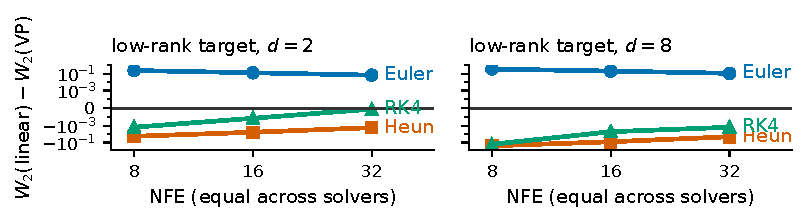
\includegraphics[width=\linewidth]{figures/fig3_interaction.pdf}
  \caption{Signed low-rank $\wtwo$ margin at equal NFE (artifact
  \artifact{A1}). Positive values prefer VP; negative values prefer
  linear; the preferred path flips with the solver. The axis is
  symmetric-log (linear threshold $10^{-4}$) since margins span four
  orders of magnitude and change sign.}
  \label{fig:interaction}
  \vspace{-6pt}
\end{figure}

\section{A minimal non-implication for fixed-grid Euler}
\label{sec:prop}

\begin{proposition}
\label{prop:euler}
Fix $L>0$ and an integer $N\ge1$; let $h=1/N$ and let forward Euler use the
left-endpoint grid $t_n=nh$ on $[0,1]$. Set
$\epsilon_N=N\{e^{L/N}-1\}-L>0$ and define $f_k(t,x)=a_k(t)x$ with
$a_0(t)=L$ and $a_{1,N}(t)=L+\epsilon_N\cos(2\pi Nt)$. For $x(0)=1$:
(i) both exact endpoints equal $e^{L}$;
(ii) $\int_0^1 a_{1,N}^2=L^2+\epsilon_N^2/2>\int_0^1 a_0^2$;
(iii) Euler is \emph{exact} for $a_{1,N}$;
(iv) Euler has strictly positive endpoint error for $a_0$.
Hence larger averaged squared Jacobian does not imply larger fixed-grid
Euler endpoint error.
\end{proposition}

\begin{proof}
(i) $\int_0^1\cos(2\pi Nt)\,dt=0$, so both coefficients integrate to $L$
and $x(1)=e^{L}$. (ii) Orthogonality gives
$\int_0^1a_{1,N}^2=L^2+\epsilon_N^2/2$, and $\epsilon_N>0$ since
$e^{z}>1+z$ for $z>0$. (iii) $\cos(2\pi Nt_n)=1$ at every node, so each
Euler factor is $1+h(L+\epsilon_N)=e^{L/N}$; the product is $e^{L}$.
(iv) $(1+L/N)^N<e^{L}$ since $\log(1+z)<z$.
\end{proof}

The quantifiers matter: $a_{1,N}$ is chosen after the grid, its
amplitude vanishes as $N\to\infty$, and shifted grids or multi-stage
solvers sample different phases. The construction shows non-implication
for fixed-grid left-endpoint Euler only---neither the mechanism behind
every Gaussian inversion nor a new numerical-analysis phenomenon; the
full proof and edge-case audit are in the supplement.

\section{Related work}
\label{sec:related}

Flow matching and stochastic interpolants define the Gaussian path
family and its fields~\citep{lipman2023flow,albergo2025stochastic,
liu2023rectified}; Lipschitz-guided schedule design proposes the
criterion we test~\citep{lipschitzguided2025}. Fast diffusion solvers
exploit exactly integrated linear parts and solver-specific
expansions~\citep{lu2022dpmsolver,lu2022dpmsolverpp,zhang2023deis}, EDM
separates schedule from discretization~\citep{karras2022edm}, and Align
Your Steps tunes schedules per solver, model, and
dataset~\citep{sabour2024align}: solver-dependent schedule quality is
known. Runge--Kutta and backward error analysis supply the local-error
machinery~\citep{butcher1963coefficients,hairer1993solving,
hairer2006geometric}; Gaussian $\wtwo$ is due to
\citet{gelbrich1990formula}. None states the commuting inversion
benchmark or the grid-aware non-implication; search absence does not
establish novelty.

\section{Limitations and conclusion}
\label{sec:limits}

Our systems are closed-form, commuting, affine Gaussian flows with two
paths, three solvers, $d\in\{2,8\}$, and small budgets, plus one
pre-registered non-centered replication family; no learned neural field
is evaluated and the proposition is grid-aware. Exponential and
exact-linear integrators solve affine fields exactly, so the result concerns
generic fixed-stage Runge--Kutta discretization. Our result does not refute Lipschitz-guided schedules as an optimization
device when the minimizer is admissible. In the tested systems the
averaged-regularity \emph{ordering} of two fixed paths does not determine
the fixed-NFE $\wtwo$ ordering, because the tested averaged-regularity
scalar does not retain the temporal information carried by solver-stage
sampling and transported signed defects. All
numerical statements map to the accompanying audit artifacts.

\bibliographystyle{plainnat}
\bibliography{references}

\end{document}
